\vspace{-2ex}
\section{Introduction}\label{sec-intro}
\vspace{-1ex}
Retrieval-Augmented Generation (RAG), as a powerful technique to improve downstream tasks by retrieving additional information from external data sources, has been successfully applied to various real-world applications~\cite{ding2024survey, gao2023retrieval, zeng2024towards, zhao2024retrieval}. In RAG frameworks, retrievers search for additional knowledge, skills, and tools based on user-defined queries or task instructions. The retrieved content is then refined by an organizer and seamlessly integrated with the original query or instruction, which is further fed into the generator to produce the final answer. For example, when conducting question-answering (QA) tasks, the classic "Retriever-then-Reader" frameworks~\cite{ju2022grape, karpukhin2020dense, xiong2020answering, zhu2021retrieving} retrieve external factual knowledge to improve the answer faithfulness, which significantly benefit social goodness and mitigate risks in high-stake scenarios (e.g., medical, legal,  financial, and education consultation~\cite{xiong2024benchmarking, xu2024ram, zhang2023enhancing}). Moreover, recent advancements in large language models (LLMs) have further underscored the power of RAG in enhancing the social responsibility of LLMs, such as mitigating hallucinations~\cite{tonmoy2024comprehensive}, enhancing interpretability and transparency~\cite{kim2024re}, enabling dynamic adaptability~\cite{shi2024retrieval, wang2023knowledge}, reducing privacy risks~\cite{zeng2024mitigating, zeng2024good}, ensuring reliability/robust responses~\cite{fang2024enhancing, xiang2024certifiably}, and promoting fair treatment~\cite{shrestha2024fairrag}.


Building on the unprecedented success of RAG and further considering the ubiquity of graphs in real-world applications~\cite{zhang2020deep}, recent research has explored the integration of RAG with graph-structured data. Unlike textual or visual data, graph-structured data encodes heterogeneous and relational information through its intrinsic "nodes connected by edges" nature. For example, individuals connected by social relationships of social networks usually exhibit homophily behaviors~\cite{mcpherson2001birds}, sequential decision-making steps in plans follow casual dependency~\cite{wu2024can}, and atoms belonging to the same functional group within a molecule possess unique structural properties~\cite{ertl2017algorithm, zang2023hierarchical}. Designing the RAG that utilizes relational information requires adapting its core components, such as the retriever and generator, to seamlessly integrate graph-structured data, resulting in GraphRAG. Different from RAG, which predominantly uses semantic/lexical similarity search~\cite{fan2024survey, gao2023retrieval}, GraphRAG offers unique advantages in capturing relational knowledge by leveraging graph-based machine learning (e.g., Graph Neural Networks (GNNs)) and graph/network analysis techniques (e.g., Graph Traversal Search and Community Detection~\cite{edge2024local, wang2024knowledge}). For example, considering the query ``What drugs are used to treat epithelioid sarcoma and also affect the EZH2 gene product?"~\cite{wu2024stark}, blindly executing the existing BM25 or embedding-based search that relies solely on semantic/lexical similarity ignores relational knowledge encoded in graph structure. In contrast, some GraphRAG methods traverse the graph along the relational path ``Disease (Epithelioid Sarcoma) $\rightarrow$ [indication] $\rightarrow$ Drug $\leftarrow$ [target] $\leftarrow$ Gene/Protein (EZH2 gene product)" to retrieve neighbors of Epithelioid Disease following the relation [indication], neighbors of Gene EZH2 following the relation [target], and find their intersected drug~\cite{jin2024graph, luoreasoning, wang2024knowledge}. Moreover, some domains involve entities with extremely complex geometry that require dedicated model design to characterize.
% \aj{incomplete sentence?Moreover, some domains involve entities with extremely complex geometry that require careful handling}. 
For example, 3D structures in molecular graphs~\cite{chen2025graph, wigh2022review} and hierarchical tree structures commonly found in product taxonomies (e.g., on Amazon~\cite{zhang2021deep}), in document sections (e.g., when using Adobe Acrobat~\cite{zhang2024tree}), and social networks (e.g., at Snap~\cite{ma2024harec}) requires carefully designed graph encoders (or, more precisely, geometric encoders) with appropriate expressiveness to capture structural nuances~\cite{ma2024harec, zhang2024hierarchical}. Simply verbalizing node texts and feeding them into LLMs cannot express complex geometric information and becomes infeasible given the exponentially growing textual descriptions as neighborhood layers expand. 



Despite the above advantages of GraphRAGs over RAGs, designing appropriate GraphRAGs faces unprecedented challenges due to the following differences in graph-structured data:



\vspace{-1ex}
\begin{itemize}[leftmargin=*]
    \item \textbf{Difference 1 - Unified versus (vs.) Diverse-Formatted Information}: Unlike conventional RAG, where semantic information can be uniformly represented as a 2D grid of image patches or a 1D sequence of textual corpora, graph-structured data often encompass diverse formats and are stored in heterogeneous sources~\cite{aggarwal2017edge, bodnar2021weisfeiler, wang2022retrieval}. For example, document graphs embed entities as sentence chunks~\cite{edge2024local, wang2024knowledge}, knowledge graphs store graph information as triplets or paths~\cite{chang2024path}, and molecule graphs consist of higher-order structures (e.g., cellular complexes)~\cite{bodnar2021weisfeiler}, as shown in Figure~\ref{fig-challenge}. Some graph data may even be multimodal (e.g., text-attributed graphs include both structural and textual attributes, and scene graphs combine structures and vision). Consequently, this diversity necessitates different RAG designs. For retrievers, conventional RAG assumes the target information is indexed in an image or text corpus, which can be uniformly represented as vector embeddings and enable one-size-fits-all embedding-based retrieval. However, retrievers for GraphRAG must consider the concrete format and source of the desired information, making the one-size-fits-all design impractical. When dealing with knowledge graph question-answering, information of nodes, edges, or subgraphs is usually fetched by graph search before embedding matching-based retrieval~\cite{wang2023knowledge, yasunaga2021qa}. This fetching operation is usually conducted by identifying relevant nodes/edges/subgraphs via entity linking, relational matching, and graph search algorithms (e.g., Breadth-First Search, Depth-First Search, Monte Carlo Tree Search, and A* search)~\cite{tian2024graph, wang2023knowledge, zhuang2023toolchain}, which is unachievable if solely through deep learning-based embedding similarity search. 
    Furthermore, the design of the retriever should ensure sufficient geometric expressiveness to capture structural nuances. For instance, when retrieving APIs from a plan graph to accomplish specific goals~\cite{shen2023taskbench, shen2024hugginggpt, wu2024can}, it is essential to equip the retriever with directional awareness. This enables the execution of APIs with resource dependencies in the correct order, preventing conflicts and avoiding invalid operations. Similarly, designing expressive retrievers capable of differentiating high-order subgraph structures, such as 6-cycle benzene versus vs. 4-star Methane, and 3-star T-junction vs. 4-square road, is essential in drug design for disease treatment~\cite{hamilton2020graph} and road construction for city planning~\cite{kocayusufoglu2022flowgen}. Beyond the retriever, the generator also requires specialized designs. When retrieved content includes complex graph structures with textual attributes, simply verbalizing the text of the subgraph and concatenating it into a prompt may obscure critical structural information. In these cases, encoding the graph with graph encoders such as GNNs before integrating it into generation can help preserve structural nuances~\cite{knowledgenavigator, unioqa, wang2022retrieval, wen2023mindmap, retrieve_rewrite_answer}.
    


    \item \textbf{Difference 2 - Independent vs. Interdependent Information:} In conventional RAG, information is stored and utilized independently. For example, documents are split into chunks, such as individual sentences, paragraphs, or a fixed number of tokens, based on the document context and downstream task~\cite{barnett2024seven, zhu2021retrieving}. Each chunk is then indexed and stored independently in a vector database. This independence prevents the retrieval from capturing chunk relations, which hinders performance on tasks requiring multi-hop reasoning and long-form planning. However, GraphRAG stores chunks as interconnected nodes with edges denoting their relations, which can benefit retrieval, organization, and generation. For retrieval, these edges could enable multi-hop traversal to capture other chunks that share a logical connection with existing retrieved chunks. Furthermore, the retrieved content can be organized not only by their semantic meaning (e.g., reranking~\cite{chen2023understanding, ivgi2023efficient, liu2024lost}) but also their structural relations (e.g., graph pruning~\cite{su2024pipenet, wang2024reasoning}). During the generation phase, squeezing interdependency (e.g., positional encoding~\cite{shomer2024lpformer, zhao2023gimlet}) to the generator would encode richer structural signals into the generated content.
    
    
    \item \textbf{Difference 3 - Domain Invariance vs. Domain-specific Information}: The relations in graph-structured data are domain-specific. Unlike images and texts, where different domains often share transferable semantics~\cite{liu2023towards, mao2024graph}, such as textures and grains in images or vocabulary defined by the tokenizer in texts, graph-structured data lacks explicit transferable units. This shared basis in images and texts lays the foundation for designing encoders with geometric invariance and enables the well-known data-scaling law. However, for graph-structured data, the underlying data generation process governing the generated graphs varies significantly across different domains. This variability makes the relational information highly domain-specific, and it is nearly impossible to design a unified GraphRAG applicable to different domains. For example, when predicting the topic of an academic paper, the widely accepted homophily assumption suggests retrieving references from the paper to inform its topic prediction~\cite{zhu2020beyond}. However, this homophily assumption is not suitable when classifying the role of an airport in a flight network, where hubs are often sparsely distributed across a country with no direct connections~\cite{cui2022positional}. Moreover, even within the same graph from the same domain, different tasks may necessitate distinct GraphRAG designs. For example, when designing an automatic email completion system to optimize communication efficiency in a company, both content relevance and tone coherence should be considered~\cite{wang2024augmenting}. To ensure the content relevance of the generated emails, one might assume that close emails (i.e., emails from the same conversation thread) share similar content and thus should be retrieved for reference. However, to maintain tone coherence, emails from staff with similar roles might be retrieved, even if they do not share close social relations (e.g., between subordinates and superiors) but instead hold similar structural roles within the company (e.g., as managers of different teams).
\end{itemize} 


\begin{figure*}[t!]
    \centering
    \includegraphics[width=1\linewidth]{Figure/rag-grag.png}
    \vspace{-3ex}
    \caption{RAG works on text and images, which can be uniformly formatted as 1D sequences or 2D grids with no relational information. In contrast, GraphRAG works on graph-structured data, which encompasses diverse formats and includes domain-specific relational information.}
    \label{fig-challenge}
    \vspace{-4ex}
\end{figure*}




Despite the above differences that have driven extensive research in GraphRAG, the current research landscape in this field remains fragmented, with significant variation in concepts, techniques, and datasets across studies. Moreover, current GraphRAG research primarily focuses on knowledge and document graphs as surveyed in Figure~\ref{fig-imbalance-pub}, often overlooking broader applications in other domains like infrastructure graphs. This imbalance not only hampers the advancement of GraphRAG but also risks creating a "bubble effect" that restricts the scope of future exploration. To address these challenges, we present a comprehensive and up-to-date review of GraphRAG, aiming to unify the GraphRAG framework from the global perspective while also specializing its unique design for each domain from the local perspective. The key contributions of this survey are as follows:

\begin{wrapfigure}{r}{0.35\textwidth}
\vspace{-0.2in}
\centering
    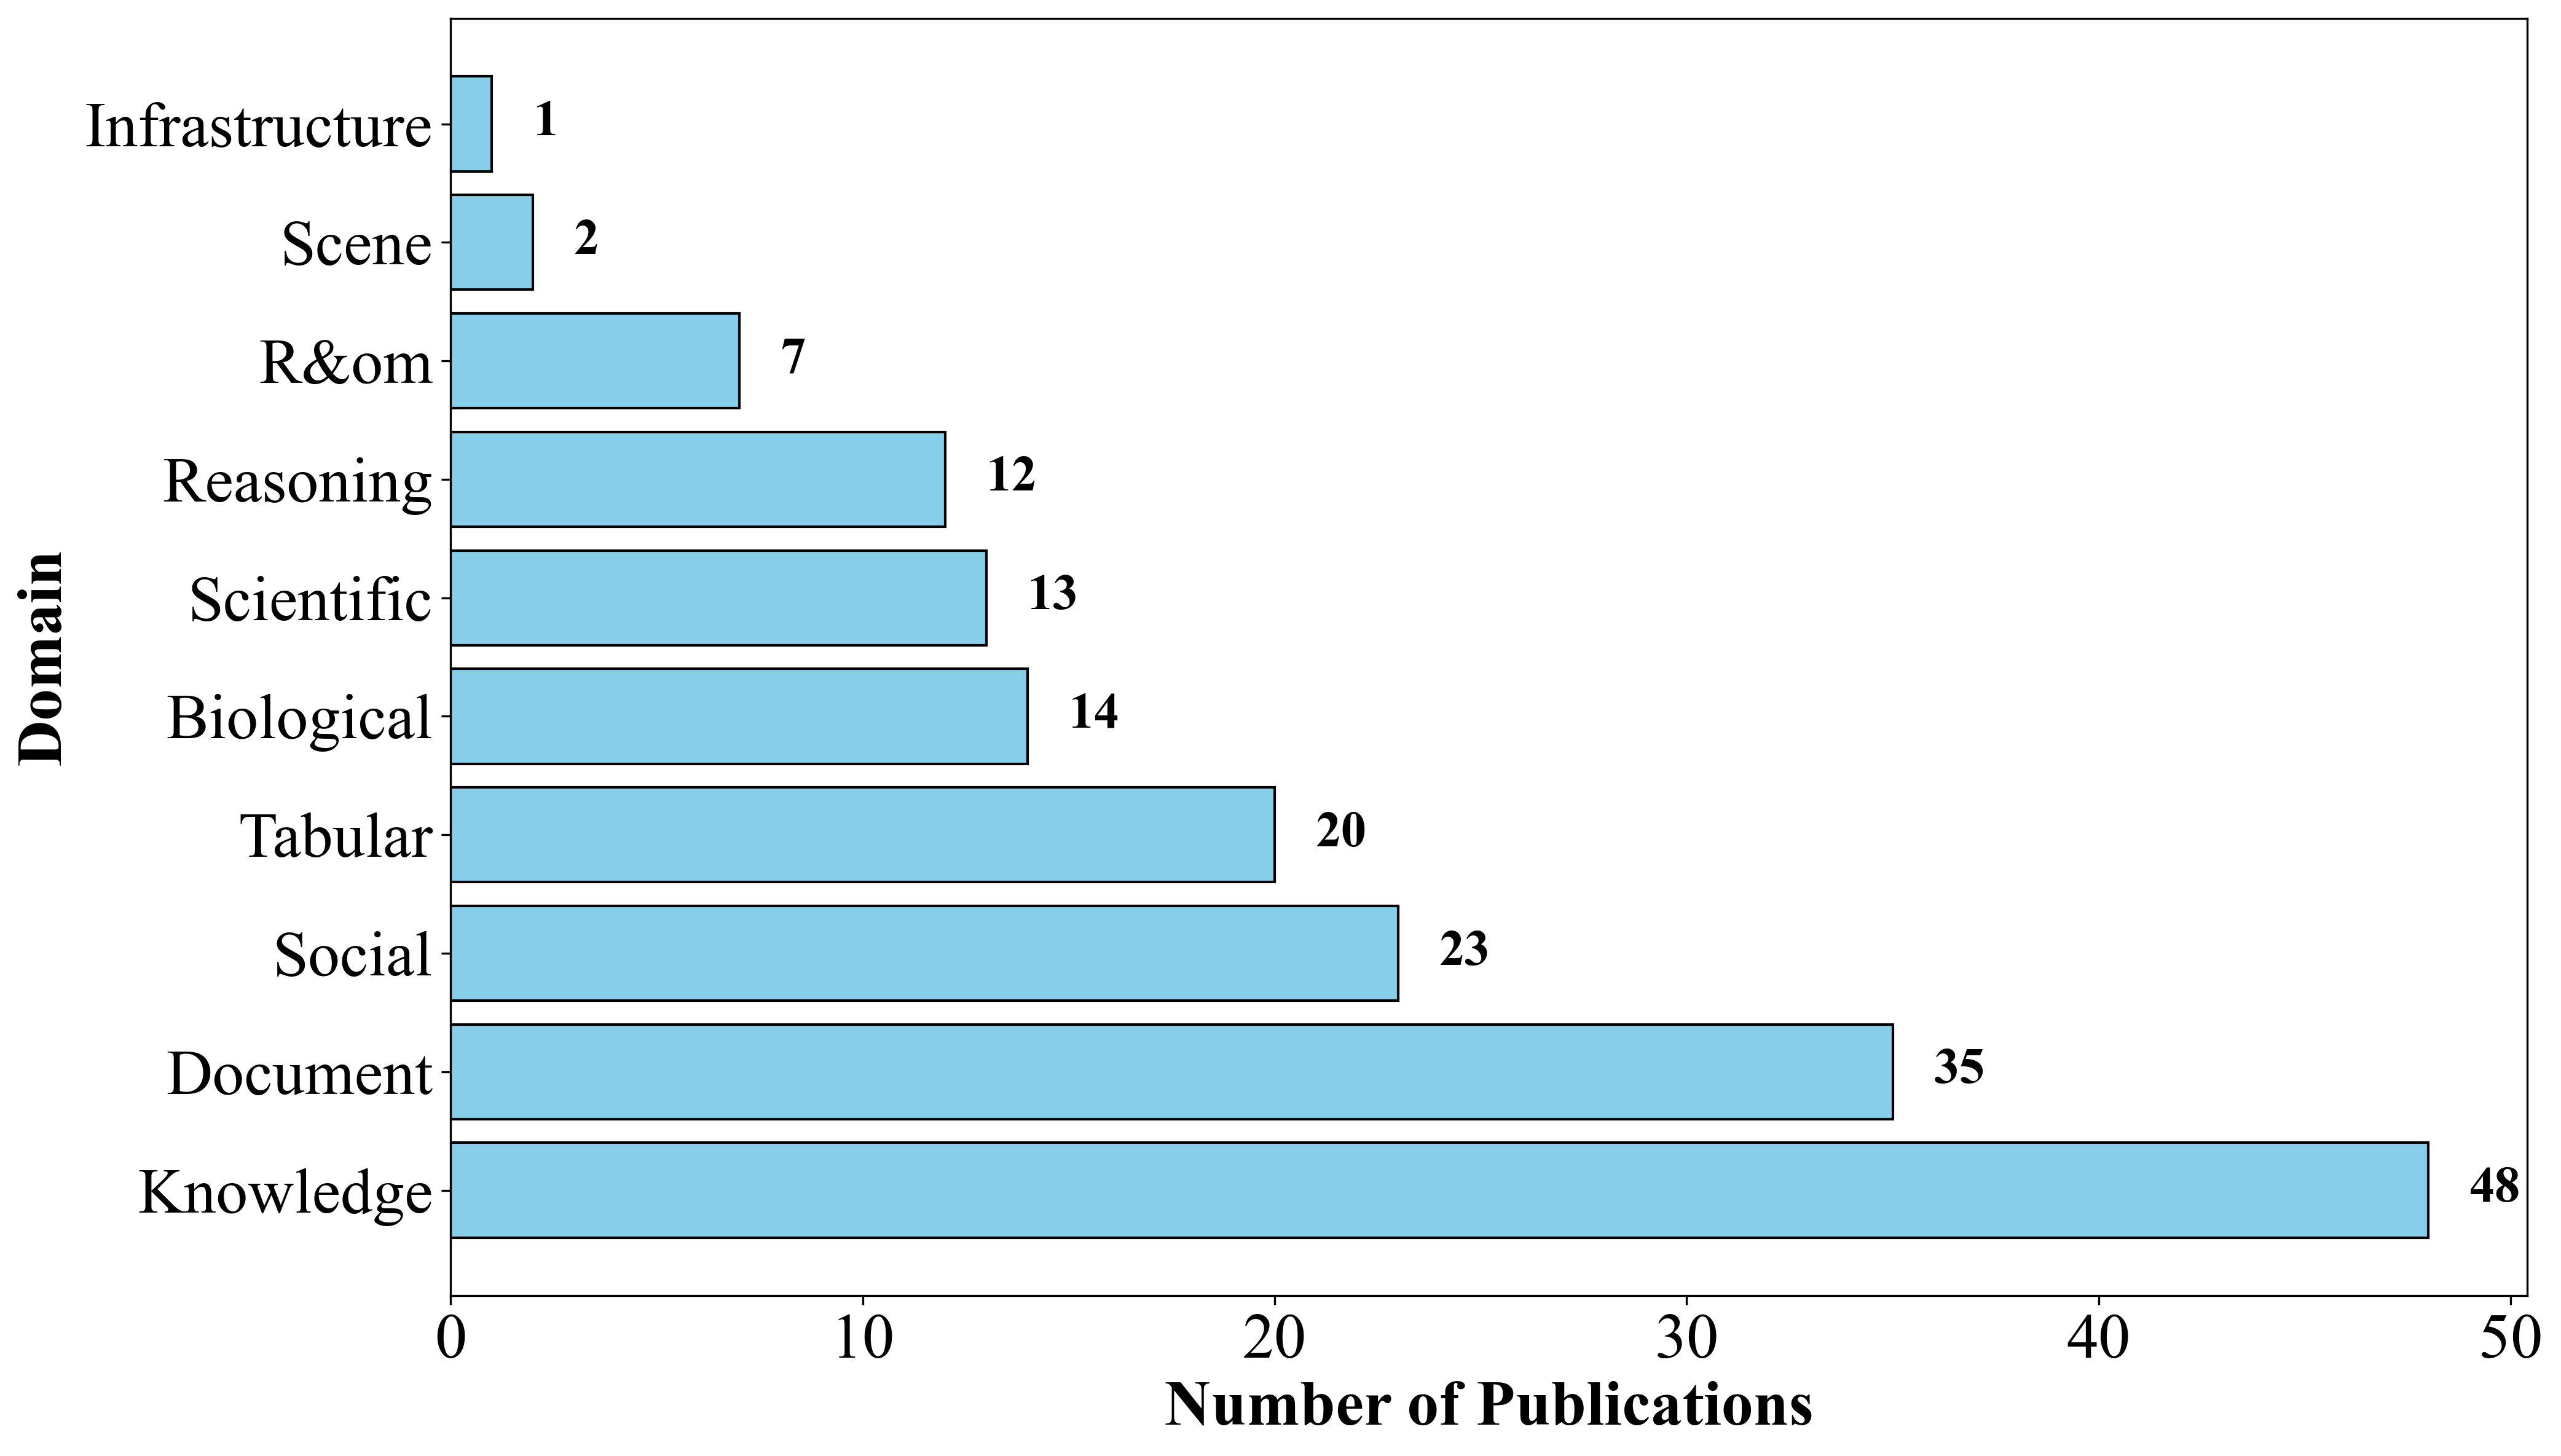
\includegraphics[width=0.35\textwidth]{Figure/count_paper_annotated.png}
    \vspace{-0.15in}
     \caption{Publications of GraphRAGs in different domains based on surveyed papers}
    \label{fig-imbalance-pub}
\vspace{-0.1in}
\end{wrapfigure}

\begin{itemize}[leftmargin=*]
    \item \textbf{A Holistic Framework of GraphRAG}: 
    We propose a holistic framework of GraphRAG consisting of five key components: query processor, retriever, organizer, generator, and graph data source. Within each component, we review representative GraphRAG techniques.

    \item \textbf{Specialization of GraphRAG in different domains}: 
    We categorize GraphRAG designs into 10 distinct domains based on their specific applications, including knowledge graph \emojikg, document graph \emojidoc, scientific graph \emojisci, social graph \emojisoc, planning \& reasoning graph \emojiplan, tabular graph \emojitab, infrastructure graph \emojiinfra, biological graph \emojibio, scene graph \emojiscene, and random graph \emojirandom. For each domain, we review their unique applications and specific graph construction methods. We then summarize the distinctive designs of each component within our proposed holistic GraphRAG framework and collect rich benchmark datasets and tool resources.
    
    \item \textbf{Challenges and Future Directions:} We highlight the challenges of current GraphRAG research and pinpoint future opportunities for further advancing GraphRAG into the new frontier.
\end{itemize}

In the following, we highlight the differences between our survey and existing surveys. Despite the urgent need for a systematic overview of GraphRAG, most existing surveys focus on general RAG within the context of i.i.d. data~\cite{asai2023retrieval, gao2023retrieval, li2022survey, zhao2024retrieval, zhou2024trustworthiness}. Before the advent of LLMs, earlier surveys focused on textual RAGs~\cite{asai2023retrieval, li2022survey}. With the recent unprecedented success achieved by foundational models such as LLMs, various surveys have explored foundational-model-powered RAG in different modalities. \citet{gao2023retrieval} group existing RAG approaches into three categories (Naive, Advanced, and Modular RAGs), summarize three core techniques (Retrieval, Generation, and Augmentation), and review evaluation metrics. In parallel, \citet{zhao2024retrieval} review representative RAG systems according to their corresponding application and data modality. \cite{zhou2024trustworthiness} focuses on reviewing trustworthy concerns and techniques of RAG. However, none of them have a dedicated focus on graph-structured data. To the best of our knowledge, only one very recent study~\cite{peng2024graph} has specifically surveyed RAG in the context of graph-structured data. However, this work mainly focuses on reviewing techniques introduced by graphs under the conventional RAG architecture without specializing in reviewing diverse relations and technical designs for graphs across different domains. In contrast to its holistic review philosophy, we recognize the inherent heterogeneity of graph-structured data and specialize our GraphRAG review across different domains. Specifically, we uncover the fundamental task applications (when to retrieve), graph construction methods and relational rationales (what to retrieve), and GraphRAG techniques (how to retrieve) for each domain. In this way, our survey provides a comprehensive overview of GraphRAG for information retrieval, data mining, and machine learning communities and domain-specific insights that facilitate interdisciplinary research and industrial opportunities.

Our survey is structured as follows: Section~\ref{sec-framework} introduces the holistic framework of GraphRAG and introduces representative techniques for its five key components. From Section~\ref{sec-kg} to \ref{sec-other}, we delve into specific domains, reviewing unique task applications, summarizing existing graph construction methods that guide GraphRAG design for that domain, highlighting domain-specific techniques for each of the five components within our proposed holistic framework, and presenting existing GraphRAG resources (e.g., benchmark datasets and tools) used across different domains. Finally, we discuss research challenges and opportunities in Section~\ref{sec-challenge} and conclude our survey in Section~\ref{sec-conclusion}.


